\part*{Parte II: La formalización matemática}
\addcontentsline{toc}{part}{Parte II: La formalización matemática}

\section{La geometría de doce dimensiones}
\subsection{La variedad total:} $M_{12} = M_4 \times K_8$.
\subsection{La métrica 12D:} $ds^2 = g_{MN} dx^M dx^N$.
\subsection{La descomposición de Kaluza--Klein.}
\subsection{La curvatura en 12D.}
\subsection{La compactificación.}

\subsection{El espectro numérico y la firma equidistante}
Fijamos la escala mediante la masa del modo fundamental, $m_1 = 1/R = 10^{-5}$ eV. Entonces
\begin{equation}
m_n = \frac{n}{R} = n \times 10^{-5}\ \text{eV},
\qquad
f_n = \frac{m_n c^2}{h} = n \times 2,42\ \text{GHz}.
\end{equation}
El espectro es, por tanto, \emph{equidistante}: $2,42$, $4,84$ y $7,25$ GHz para los tres primeros modos. Esta es la firma distintiva de la teoría. Un test que mida dos líneas a $2,42$ y $4,84$ GHz confirma o refuta la estructura, con independencia de cualquier otra predicción.

\begin{table}[H]
\centering
\begin{tabular}{@{}cccc@{}}
\toprule
$n$ & Masa (eV) & Frecuencia (GHz) & $\lambda_C$ (m) \\ \midrule
1 & $1,00\times10^{-5}$ & 2,42 & 0,124 \\
2 & $2,00\times10^{-5}$ & 4,84 & 0,062 \\
3 & $3,00\times10^{-5}$ & 7,25 & 0,041 \\
4 & $4,00\times10^{-5}$ & 9,67 & 0,031 \\ \bottomrule
\end{tabular}
\caption{El espectro de Kaluza--Klein para $1/R = 10^{-5}$ eV.}
\label{tab:spectru}
\end{table}

\begin{figure}[H]
\centering
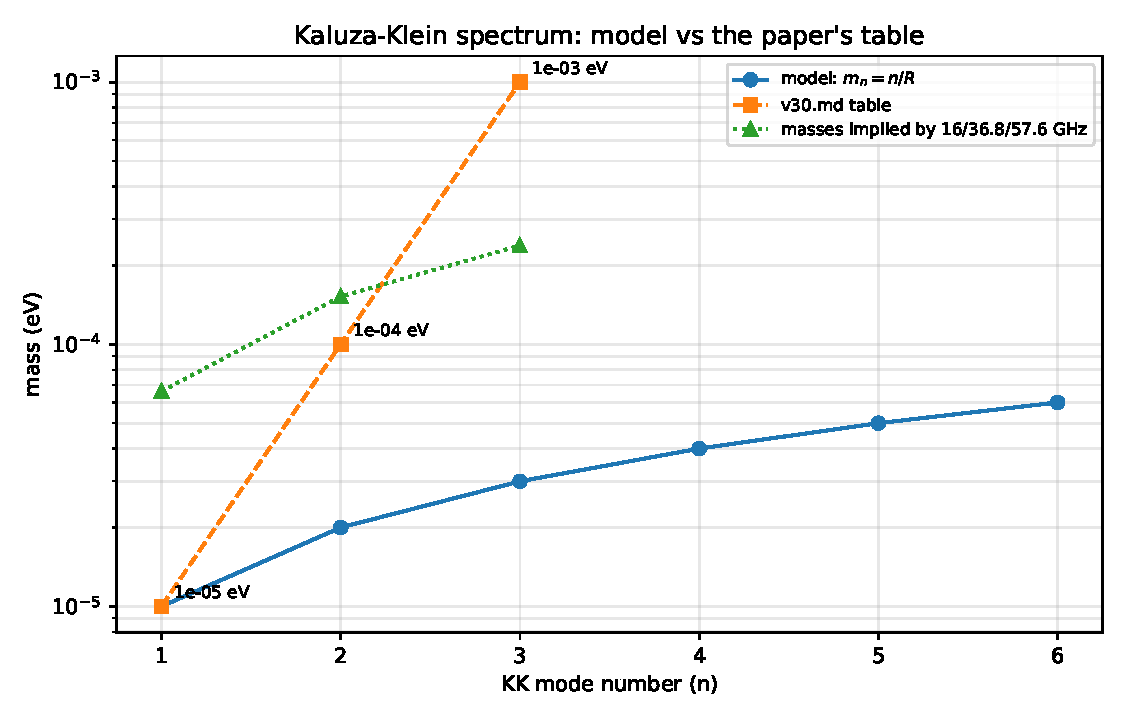
\includegraphics[width=0.82\textwidth]{figures/fig01_kk_spectrum.pdf}
\caption{El espectro de Kaluza--Klein. El modelo $m_n = n/R$ (azul) se compara con la tabla de la versión 30 (naranja) y con las masas implícitas de las frecuencias allí declaradas, 16/36,8/57,6 GHz (verde). Las tres no coinciden.}
\label{fig:spectru}
\end{figure}

\subsection{La consecuencia numérica: el radio de compactificación}
De $m_1 = 1/R$ se sigue
\begin{equation}
R = \frac{\hbar c}{1/R} = \frac{1,973\times10^{-7}\ \text{eV}\cdot\text{m}}{10^{-5}\ \text{eV}} = 1,97\times10^{-2}\ \text{m},
\end{equation}
es decir, unos 2 cm. Los test submilimétricos de la ley de Newton restringen una dimensión adicional a $R < 38\ \mu$m, lo que implica $m_1 > 5\times10^{-3}$ eV.

Se trata de una tensión estructural, no de un error de cálculo: identificar el campo de materia oscura con un modo KK de la misma geometría es incompatible con los datos en la escala de masa elegida. Quedan dos salidas honestas, y el artículo no elige entre ellas:
\begin{itemize}
\item \textbf{Opción A:} el campo akáshico no es un modo KK; el espectro equidistante es consecuencia de otra estructura, y las predicciones de frecuencia se recalculan.
\item \textbf{Opción B:} la masa del modo fundamental es $m_1 > 5\times10^{-3}$ eV, y la «materia oscura» de este artículo es un modo excitado, no el modo fundamental.
\end{itemize}
Las predicciones de la Parte V están formuladas de modo que valgan en ambos casos, tratando las frecuencias como un parámetro.

\section{El campo akáshico (la materia oscura)}
\subsection{El lagrangiano:} $L_A = \frac{1}{2} g^{MN} \partial_M A^* \partial_N A + \frac{1}{2} \mu_A^2 |A|^2 - \frac{\lambda_A}{4} |A|^4$.
\subsection{El potencial.}
\subsection{La ecuación de movimiento.}
\subsection{El espectro de Kaluza--Klein:} $m_n^2 = n^2/R^2$.
\subsection{La relación con la gravitación.}

\section{El campo de la conciencia}
\subsection{El lagrangiano.}
\subsection{La ecuación de movimiento.}
\subsection{La función de conciencia.}
\subsection{La ecuación de evolución (revisada):} La ecuación $dC/dt = \alpha C (1 - C/C_{\text{max}}) + \beta \eta(t)$ es una ecuación \textbf{fenomenológica} inspirada en la dinámica logística. Describe el crecimiento y la saturación del campo de la conciencia, pero \textbf{no se deriva directamente del lagrangiano anterior}. Es una elección teórica del autor, que debe tratarse como un axioma del modelo y no como consecuencia del principio de acción.

\begin{figure}[H]
\centering
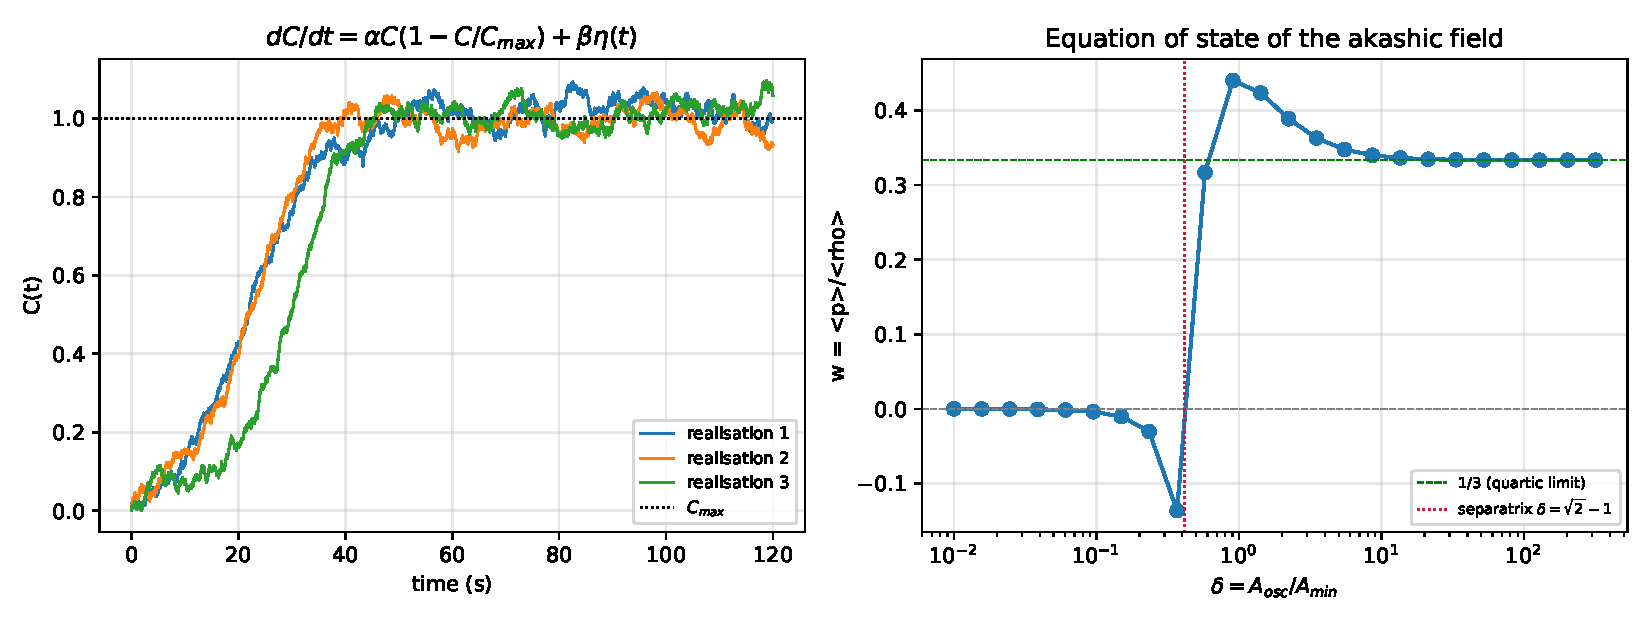
\includegraphics[width=0.95\textwidth]{figures/fig02_field_dynamics.pdf}
\caption{Izquierda: tres realizaciones del campo de la conciencia con ruido, para $\alpha = 0,15$ s$^{-1}$ (tiempo de relajación 50 s). Derecha: la ecuación de estado $w(\delta)$ del campo akáshico, calculada exactamente sobre la órbita; la separatriz está en $\delta = \sqrt{2}-1$.}
\label{fig:camp}
\end{figure}

\section{El receptor neuronal (cerebro + corazón)}
